
%(BEGIN_QUESTION)
% Copyright 2010, Tony R. Kuphaldt, released under the Creative Commons Attribution License (v 1.0)
% This means you may do almost anything with this work of mine, so long as you give me proper credit

Suppose you need to measure the current drawn by an AC electric motor, but you do not have an AC ammeter with a high enough measurement range to measure the motor's current (approximately 15 to 27 amps).  Your only AC ammeter only registers as high as 3 amps.

However, you do have a transformer in your shop with a 240:24 volt step-down ratio (10:1).  Sketch the necessary wire connections to use this transformer to step down the motor's current to a level your AC ammeter can read.  If you need to break the motor power circuit in any location, mark the intended break with an ``X'':

$$\includegraphics[width=15.5cm]{i03735x01.eps}$$

\underbar{file i03735}
%(END_QUESTION)





%(BEGIN_ANSWER)

$$\includegraphics[width=15.5cm]{i03735x02.eps}$$

%(END_ANSWER)





%(BEGIN_NOTES)

{\bf This question is intended for exams only and not worksheets!}.

%(END_NOTES)

